\section{Objetivo del Proyecto}
\begin{itemize}
	\item Programa ambiental para la recuperación de fuentes hídricas de la ciudad de Popayán dirigido por la Alcaldía. El programa consta de campañas educativas dirigidas a las comunidades aledañas a las fuentes hídricas, inversión en un PTAR para manejo de residuos líquidos.
	\item Implementación de mecanismos para la evaluación regular de la calidad del agua
	\item Sanciones con base a las normativas de la ciudad a quienes arrojen residuos a los ríos en acompañamiento con la policía ambiental, para así concientizar a la población del daño que se está ocasionando al medio ambiente
	\item Monitoreo constante sobre las zonas de mayor relevancia en las cuales la población urbana tienda a contaminar.
	\item Búsqueda de métodos químicos que permitan la depuración de las aguas contaminadas por concentraciones bacteriológicas que son dañinas para el ecosistema.
	\item Identificación de tecnologías que nos permitan extraer desechos de todo tipo tanto solidos como orgánicos, el cual identifique y recolecte amenazas para el ambiente y la salud de la población que vive en la zona.
	\item Planes de gestión de desechos, en los cuales se organice de manera adecuada la manipulación de y evacuación de dichos desechos.
	\item Estructurar un grupo que se encargue de la gestión ambiental en la ciudad de Popayán
	\item Buscar fundaciones internacionales que apoyen el cuidado del medio ambiente para que brinden información, experiencia, y capacitación.
	\item Explorar actividades que involucren a la población para fomentar el interés, conocimientos y reflexión del cuidado de estas fuentes de vida.
	\item Aumentar señalizaciones informativas que atraigan la atención de las personas.
	\item Lograr un acercamiento con el gobierno para que apoye los proyectos de interés ambiental.
	\item Usar nutrientes y plaguicidas naturales
	\item Desarrollar un mejor sistema para el tratamiento de las aguas residuales
	\item Acabar con la deforestación
	\item Actividades agropecuarias más amigables con los ríos y el ambiente en general
	\item Reducción del uso de aceites y baterías
	\item Disminuir el consumo de plásticos
\end{itemize}

\begin{figure}[H]
	\centering
	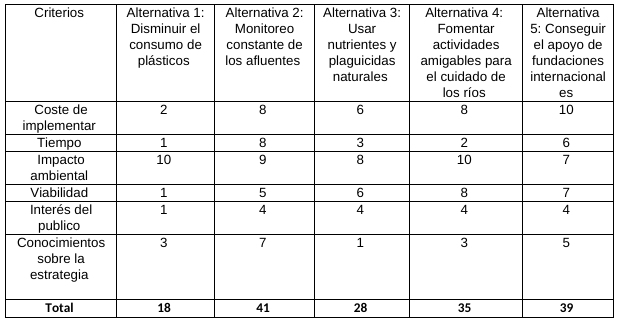
\includegraphics[width=0.7\textwidth]{codigofuente/pgf/alternativas}
	\caption{Tabla de filtros de alternativas.}
	\label{fig:alt}
\end{figure}
